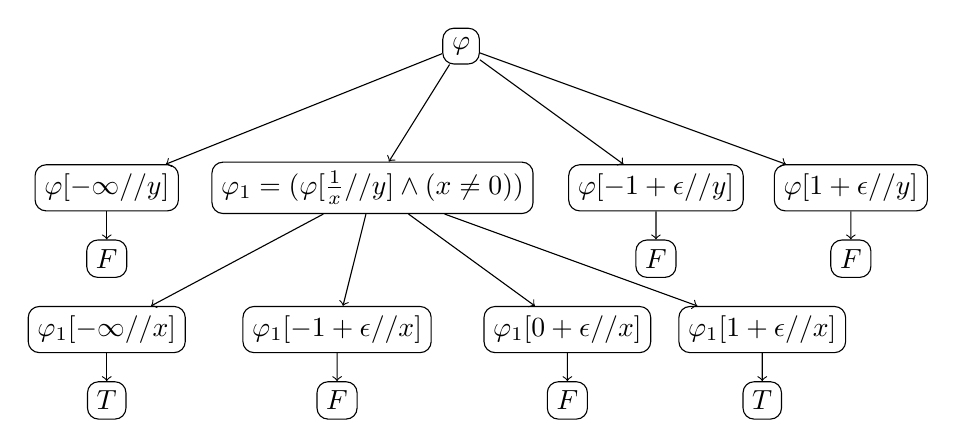
\begin{tikzpicture}[scale=0.9, 
				    state/.style={draw, rounded corners, fill=none,
				    			  text centered, text=black}]
	\node[state] (u1) at (5, 7) {$\varphi$};
	\node[state] (u2) at (0, 5) {$\varphi[-\infty//y]$};
	\node[state] (u3) at (3.75, 5) {$\varphi_{1}=(\varphi[\frac{1}{x}//y]\wedge (x\neq0))$};
	\node[state] (u4) at (7.75, 5) {$\varphi[-1+\epsilon//y]$};
	\node[state] (u5) at (0, 4) {$F$};
	\node[state] (u6) at (10.5, 5) {$\varphi[1+\epsilon//y]$};
	\node[state] (u7) at (0, 3) {$\varphi_{1}[-\infty//x]$};
	\node[state] (u8) at (3.25, 3) {$\varphi_{1}[-1+\epsilon//x]$};
	\node[state] (u9) at (6.5, 3) {$\varphi_{1}[0+\epsilon//x]$};
	\node[state] (u15) at (9.25, 3) {$\varphi_{1}[1+\epsilon//x]$};
	\node[state] (u10) at (7.75, 4) {$F$};
	\node[state] (u11) at (10.5, 4) {$F$};
	\node[state] (u12) at (0, 2) {$T$};
	\node[state] (u13) at (3.25, 2) {$F$};
	\node[state] (u14) at (6.5, 2) {$F$};
	\node[state] (u16) at (9.25, 2) {$T$};
	
	\path[->] 	(u1)  edge   (u2);
	\path[->] 	(u1)  edge   (u3);
	\path[->] 	(u1)  edge   (u4);
	\path[->] 	(u1)  edge   (u6);
	\path[->] 	(u2)  edge   (u5);
	\path[->] 	(u3)  edge   (u7);
	\path[->] 	(u3)  edge   (u8);
	\path[->] 	(u3)  edge   (u9);
	\path[->] 	(u4)  edge   (u10);
	\path[->] 	(u6)  edge   (u11);
	\path[->] 	(u8)  edge   (u13);
	\path[->] 	(u7)  edge   (u12);
	\path[->] 	(u9)  edge   (u14);
	\path[->] 	(u3)  edge   (u15);
	\path[->] 	(u15)  edge   (u16);

\end{tikzpicture}
